\chapter{Diagnostic de l'image}
\label{chap:chapter_4}
\chapterintro
Comme évoqué durant le préambule, cette partie s'intéresse au premier niveau de diagnostic, c'est à dire celui de l'image sur données \gls{rcm}. La séparation sur problématique binaire, malin et non malin, sera ainsi évaluée mais également sur trois classes avec d'une part les tissus sains, bénin et malin.\par

Ainsi, plusieurs aspects se distinguerons dans ce chapitre dont l'extraction de caractéristiques pertinentes par méthodes manuelles et auto déterminée et l'utilisation de méthodes de classification éprouvées. Nous nous intéresserons également à l'influence de divers paramètres liés à la normalisation des caractéristiques, à la réduction de l'information dans le cadre des méthodes sur base d'apprentissage par transfert et enfin sur l'influence des données sur les résultats obtenus.\par	
\newpage

%%%%%%%%%%%%%%%%%%%%%%%%%%%%%%%%%% 
%%%%%%%%%%%%%%%%% METHODOLOGIE
\section{Méthodologie}
La classification de la peau par méthode d'apprentissage est un problème très largement développée dans la littérature, notamment pour le mélanome. Néanmoins, dans le cadre de la détection du \gls{lm}/\gls{lmm} sur base d'images \gls{rcm},
cette problématique n'a été abordé que par quelques articles~\cite{Halimi2017a, Halimi2017b, Wiltgen2008, Koller2011}. Nous nous intéresserons à la détection de cette pathologie au sein de la base d'image mise à disposition, et nous étudierons cette problématique selon divers angles d'approche: 
\begin{inlinerate}
    \item la séparation entre les tissus malin et le reste des tissus (problématique à 2 classes),
    \item la séparation entre les tissus pathologiques  et les tissus qualifiés de sains (problématique à 2 classes),
    \item et enfin la séparation des tissus malins, bénins et sains (problématique à 3 classes).
\end{inlinerate}\par

Afin de traiter ces problématiques, nous aborderons ces cas à l'aide de mécaniques liées à l'apprentissage supervisé, que nous déroulerons lors de prochains paragraphes. En effet, ces mécaniques ont largement été employé et démontrée fonctionnelles dans des problèmes similaires de classification d'images médicales. Dans un premier temps, nous décrirons le processus par apprentissage automatique ( voir \Cref{fig:scheme_macro_pipeline} - en haut): nous décrirons bloc par bloc les traitements proposés de l'extraction de caractéristique à l'étape de classification. Dans un second temps, nous décririons le processus d'apprentissage profond ( voir \Cref{fig:scheme_macro_pipeline} - en bas): nous traiterons de l'augmentation des données et proposerons une méthodologie d'entraînement. Enfin, nous terminerons par une descriptions des résultats obtenus, tenterons d'expliquer ces derniers, et déterminerons les choix les plus cohérents pour la suite.\par

\begin{figure}[H]
\centering
    \includegraphics[width=\linewidth]{contents/chapter_4/resources/scheme_macro_pipeline_machine.pdf}
    \caption{Représentation macroscopique du processus de diagnostic image suivi dans le cadre de l'apprentissage automatique.}
    \label{fig:scheme_macro_pipeline}
\end{figure}\par

Cette section se destine à présenter l'ensemble des étapes consacrée à la classification des images de \gls{rcm} selon un processus d'apprentissage automatique. Celui-ci se décompose en quatre étapes majeures:
\begin{inlinerate}
    \item l'extraction de caractéristiques,
    \item le balancement des données,
    \item le post-traitement,
    \item et la classification
\end{inlinerate}.
Le pré traitement des images n'est pas considéré car jugé peu utile sur ces dernières. Ce processus sera décrit point par point lors des prochaines sous-parties.\par
\newpage

%%%%%%%%%%%%%%%%%%%%%%%%%%%%%%%%%% 
%%%%%%%%%%%%%%%%% FEATURES
\section{Extraction de caractéristiques}
\label{chap:feature_extraction}
L'étape d'extraction de caractéristiques consiste en l'obtention de valeurs dérivées à partir des données brute dans le but de quantifier un phénomène jugée pertinent pour la suite du traitement (généralement de la classification). Les éléments présentés en \Cref{chap:preamble_microscopy} portent à montrer l'importance des motifs de tissus, très variables selon:
\begin{itemize}
    \item la profondeur d'acquisition : l'épiderme, \gls{dej} et le derme sont très différents du point des tissus,
    \item la pathologie à identifier : les différentes lésions en notre possession sont assez différentes selon leur états bénin ou malin.
\end{itemize}\par

Les nombreux échanges menés auprès des spécialistes en dermatologie ont également abouti sur une importance des aspects des textures au sein de leur processus cognitifs de décision vis à vis des pathologies de \gls{lm}/\gls{lmm}.\par

Nous traiterons des techniques d'extraction de caractéristiques appliquée à notre thématique, que nous aborderons selon deux axes:
\begin{inlinerate}
    \item d'une part les techniques d'extraction de caractéristiques manuelles,
    \item d'autre part les techniques d'extraction de caractéristiques non manuelles
\end{inlinerate}. Ces termes ont été utilisés suite à l'apparition de réseaux de convolution profonds, afin de catégoriser ces deux types d'approches~\cite{Nanni2017}.\par

L'extraction de caractéristiques est une problématique qui a été traitées sous deux aspects distincts: l'une par utilisation du domaine spatial et l'autre par utilisation du domaine fréquentiel. Ainsi, ces prochaines lignes traiterons la problématique dans cet ordre respectif.\par

\subsection{Extraction de caractéristiques manuelles spatiales}
L'extraction sur base d'information du domaine spatial est un champs de travail assez développé présentant comme avantage d'être intuitif mais pouvant être affecté par le bruit et distorsions. Ces opérations spatiales peuvent être décrites à deux niveaux: les descripteurs de premier ordre ne prenant en compte que les valeurs d'intensités initiales et est indifférent aux information de voisinage; et les descripteurs de second ordre et plus, prenant en compte la relation d'une valeur locale et de son voisinage~\cite{Kamila2015}.\par

Les descripteurs de premier ordre s'appliquent ainsi aux valeurs d'intensité ou à la distribution de celle-ci, sans traitement préalable. La \Cref{tab:first_order_descriptors} recense la plupart des ces mesures. Néanmoins, ces mesures tendent à ressortir des phénomènes globaux de l'image mais ne suffisent pas à elles seules à analyser  des motifs présent, mais peuvent constituer un bon complément ~\cite{Tomita1990, Srinivasan2008, Uyun2013, NyeinNyeinHlaing2015}.\par

\begin{table}[H]
    \centering
    \begin{tabular}{ll}
        \toprule
        \textbf{Mesure}             & \textbf{Formule}                                                              \\ \hline
        Moyenne                     & $\overline{x} = {1 \over n} \sum_{i=1}^n{x_i}$                                \\   
        Variance                    & $\overline{x} = \frac{1}{n}\sum_{i=1}^n x_i$                                  \\ 
        Entropie                    & \\
        Kurtosis (Courbure)         & \\
        Asymétrie                   & $\gamma_1 = \mathbb{E} \left[ \left( \frac{X - \mu}{\sigma} \right)^3 \right]$\\  
        \bottomrule
    \end{tabular}
    \caption{Liste de différentes mesures obtenues à partir du premier ordre.}
    \label{tab:first_order_descriptors}
\end{table}\par

Les descripteurs de second ordre, ou plus, utilisent l'information locale et en déduisent une relation à leur voisinage par l'utilisation généralement d'une transformation intermédiaire. Parmi ces transformation, les plus courantes sont: 
\begin{inlinerate}
    \item \gls{glcm},
    \item \gls{glrlm},
    \item et \gls{glszm}.
\end{inlinerate} 
L'extraction sur la base d'information du second ordre à notamment été traitée en 1973 pour de la reconnaissance d'image aérienne et satellites, par Robert Haralick~\cite{Haralick1973}. Ce travail est une extension des \gls{glcm}, dont le principe consiste en un recensement des combinaisons d'intensité présentent dans une image. Cette extraction nécessite une direction dans laquelle les combinaisons seront recherchées, en 2D ces directions sont aux nombre de quatre:
\begin{inlinerate}
    \item horizontale,
    \item verticale,
    \item et les deux diagonales opposées
\end{inlinerate}. Le principe de fonctionnement des \gls{glcm} est schématisé en \Cref{fig:scheme_principle_GLCM} pour une extraction selon la direction horizontale. Le travail~\cite{Haralick1973} à ainsi démontré la pertinence des \gls{glcm} dans la différenciation d'images texturés, en calculant quatorze critères statistiques selon les quatre directions évoqué précédemment. La \Cref{tab:haralick_descriptors} met à disposition les diverses mesures utilisées et formules associées. Afin de réaliser ces diverses extraction de manière optimum, nous nous référé à la bibliothèque logicielle "Mahotas"~\cite{coelho2012} proposant ces diverses mesures de manière optimisée.\par
 
\begin{figure}[H]
    \centering
    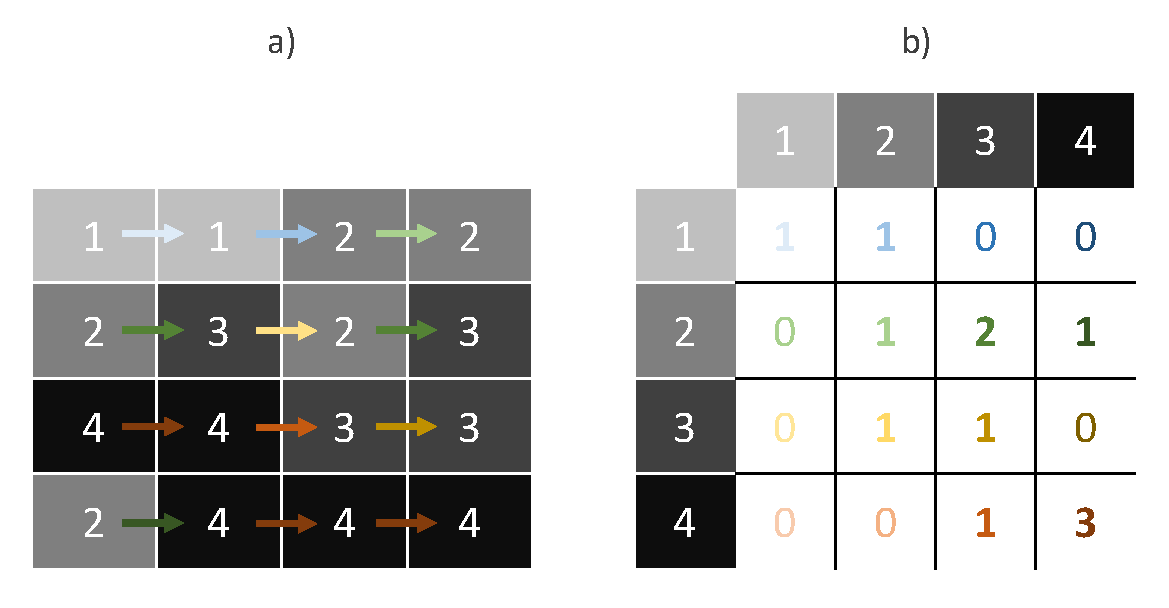
\includegraphics[width=0.8\linewidth]{contents/chapter_4/resources/scheme_principle_GLCM.pdf}
    \caption{Représentation de la création d'une matrice sur base de \gls{glcm} selon la direction horizontale.}
    \label{fig:scheme_principle_GLCM}
\end{figure}\par

L'un des travaux menée par une étude sur les lésions mélanocytaire en \gls{rcm} vont dans le sens de ces deux formes d'information~\cite{Wiltgen2008}. En effet, l'étude met en avant l'importance des douze première caractéristiques énoncés par Haralick et adjoint cinq mesure de premier ordre comme complément d'information dont :
\begin{inlinerate}
    \item la moyenne,
    \item l'erreur quadratique moyenne,
    \item l'asymétrie de la répartition de l'histogramme,
    \item le kurtosis (mesure d'aplatissement de la distribution),
    \item et l'entropie.
\end{inlinerate}
De plus, afin de rendre les caractéristiques d'Haralick plus robuste aux rotations et par la même de réduire la quantité d'information, les auteurs préconise l'utilisation d'une moyenne sur les quatre directions, dont résulte un unique vecteur de taille 1$\times$12~\cite{Wiltgen2008}.\par

\begin{table}[H]
    \centering
    \begin{tabular}{ll}
        \toprule
        \textbf{Nom}                & \textbf{Formule}                                                                              \\ \hline
        Angular Second Moment       & $ \sum_i\sum_jp(i,j)^2$                                                                       \\
        Contrast                    & $\sum_{k=0}^{N_g-1} k^2 p_{x-y}(k)$                                                           \\
        Correlation                 & $\frac{\Large{\sum_{i=1}^{N_g}\sum_{j=1}^{N_g}} (ij)p(i,j) - \mu_x\mu_y}{\sigma_x\sigma_y}$   \\
        Sum of Squares: Variance    & $\sum_{i=1}^{N_g}\sum_{j=1}^{N_g} (i - \mu)^2 p(i,j)$                                         \\
        Inverse Difference Moment   & $\sum_{i=1}^{N_g}\sum_{j=1}^{N_g} \frac{1}{1 + (i - j)^2} p(i,j)$                             \\     
        Sum Average                 & $\sum_{i=2}^{2N_g} i p_{x+y}(i)$                                                              \\    
        Sum Variance                & $\sum_{i=2}^{2N_g} (i - f_8)^2 p_{x+y}(i)$                                                    \\    
        Sum Entropy                 & $\sum_{i=2}^{2N_g} (i - f_8)^2 p_{x+y}(i)$                                                    \\    
        Entropy                     & $-\sum_{i=1}^{N_g}\sum_{j=1}^{N_g} p(i,j) \log(p(i,j))$                                       \\    
        Difference Variance         & ${\rm variance \ of ~} p_{x-y}$                                                               \\    
        Difference Entropy          & $-\sum_{i=0}^{N_g-1} p_{x-y}(i) \log(p_{x-y}(i))$                                             \\
        Measure of Correlation 1    & $\frac{f_9 - HXY1}{\max(HX,HY)}$                                                              \\  
        Measure of Correlation 2    & $[1 - \exp(-2(HXY2 - f_9))]^{1/2}$                                                            \\ 
        Maximal Correlation Coefficient    & $({\rm second \ largest \ eigenvalue \ of ~} Q)^{1/2}$ $\sum_k \frac{p(i,k)p(j,k)}{p_x(i)p_y(k)}$ \\ 
        \bottomrule
    \end{tabular}
    \caption{Liste des des différentes mesures proposé par Robert Haralick applicable aux \gls{glcm}.}
    \label{tab:haralick_descriptors}
\end{table}\par
 
Les expériences menées sur base de descripteurs manuels spatiaux se décomposerons en plusieurs temps. Tout d'abord, nous procéderons à une étude de l'importance séparée des mesures sur l'information de premier ordre et sur les mesures proposée par Haralick sur l'information de second ordre. Nous profiterons de l'expérience pour mesurer l'impact de la moyenne dans cette tâche. Dans un second temps, nous réemploierons la démarche de combinaison conjointe de ces mesures menée par l'un des articles~\cite{Wiltgen2008}. Par ailleurs, la \Cref{tab:number_features_spatial} synthétise l'ensemble des méthodes d'extraction ainsi que le nombre associé de caractéristiques extraites.\par
\begin{table}[h]
    \centering
    \begin{tabular*}{0.6\linewidth}{l@{\extracolsep{\fill}}l}
        \toprule
        \textbf{Méthode}                            & \textbf{Nombre}   \\ \hline
        Mesures premier ordre                       & 14                \\ \hline
        Haralick~\cite{Haralick1973} - 4 directions & 56                \\ \hline
        Haralick~\cite{Haralick1973} - Moyenne      & 14                \\ \hline
        Wiltgen~\cite{Wiltgen2008} - Spatial        & 17 (12+5)         \\
        \bottomrule
    \end{tabular*}
    \caption{Nombre de caractéristiques extraites par méthodes manuelles spatiale.}
    \label{tab:number_features_spatial}
\end{table}

\subsection{Extraction de caractéristiques manuelles fréquentielles}
L'extraction sur base d'information du domaine fréquentiel est également un champs de travail assez développé, notamment pour sa robustesse face au perturbation telle que le bruit, ainsi que la vitesse d'exécution de certaines opérations telle que le filtrage. En revanche, l'information extraites est moins évocatrice et nécessite une information spatiale initiale suffisante pour être juste~\cite{Kamila2015}. Plusieurs courants majeurs de représentation sont utilisés: 
\begin{itemize}
    \item la Transformée de Fourier~\cite{Ursani2007, Smach2008a},
    \item la Transformée en cosinus discrète~\cite{Sorwar2001},
    \item la Transformée en ondelettes~\cite{Arivazhagan2003,Hong2010},
    \item et la Transformée de Gabor~\cite{Ursani2007}.
\end{itemize}
Notre travail se consacrera à deux de ces approches, la transformée de Fourier et à la transformée en ondelettes, toutes deux traités sur une problématique similaire~\cite{Wiltgen2008,Halimi2017a,Halimi2017b}. Également, ces deux méthodes sont deux représentants majeures des deux grandes familles de représentation en fréquence.\par

La transformée de Fourier se résume à la décomposition d'une donnée en une somme de fréquences. Dans le cas d'une image, cette transformation donne lieu à une représentation, dans lesquelles: les basses fréquences, au centre, représentent une forme d'homogénéité au sein d'une image; tandis que les hautes fréquences, en extérieur, sont associées à de fortes transitions. Cet espace est donc approprié à la caractérisation d'image texturées, et à suscité un intérêt au milieu des années 1980~\cite{Persoon1986}. En revanche, bien que cette représentation permette de décrire parfaitement la composition fréquentielle de l'image, elle ne peut en localiser la provenance exacte~\cite{Wiltgen2008}. Différentes  mesures ont été proposés dans cet espaces afin de caractériser des textures:
\begin{itemize}
    \item l'extraction d'information à partir \textbf{de cercles concentriques} réguliers~\cite{Smach2008a, Wiltgen2008} afin d'isoler l'information propre à chaque intervalle de fréquences (\Cref{fig:scheme_fourier_features} - a),
    \item l'extraction d'information à partir \textbf{de directions} en partance du centre vers l'extérieur de la transformée à angles constants ~\cite{Wiltgen2008} (\Cref{fig:scheme_fourier_features} - b).
\end{itemize}
Ces deux travaux préconise l'extraction d'une moyenne, voire d'une déviation standard~\cite{Smach2008a, Wiltgen2008}. La transformée de Fourier sera effectuée dans le reste de ce travail par la bibliothèque logicielle "SciPy" \cite{Virtanen2020}.\par\par

\begin{figure}[h]
    \begin{center}
        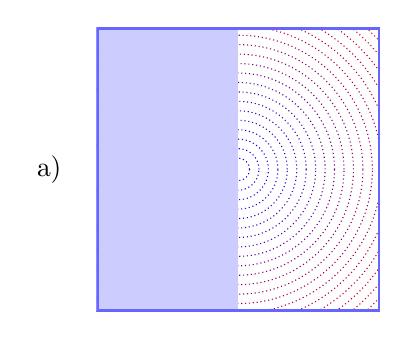
\begin{tikzpicture}[scale=1.2]
            \node[] at (-2, 0) {a)};
            \begin{scope}
                \clip (-1.5, -1.5) rectangle (1.5, 1.5);
                \foreach \cRadius in {1, ..., 22}
                    \pgfmathsetmacro\cColor{\cRadius/22*100}
                    \draw[red!\cColor!blue, densely dotted] (0, 0) circle (0.02+\cRadius*0.1); 
                    
                \fill[blue!20] (-1.5, -1.5) rectangle (0, 1.5);
                \draw[blue!60, ultra thick] (-1.5, -1.5) rectangle (1.5, 1.5);
            \end{scope}
        \end{tikzpicture}
        \qquad
        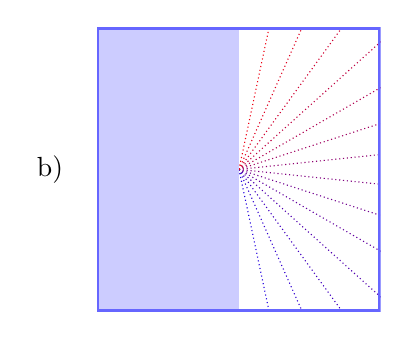
\begin{tikzpicture}[scale=1.2]
            \node[] at (-2, 0) {b)};
            \begin{scope}
                \clip (-1.5, -1.5) rectangle (1.5, 1.5);
                \foreach \cAngle in {1, ..., 16}
                    \pgfmathsetmacro\cColor{\cAngle/16*100}
                    \draw[red!\cColor!blue, densely dotted] (0, 0) -- (\cAngle* 180 / 15 -102:3); 
                \fill[blue!20] (-1.5, -1.5) rectangle (0, 1.5);
                \draw[blue!60, ultra thick] (-1.5, -1.5) rectangle (1.5, 1.5);
            \end{scope}
        \end{tikzpicture}
    \end{center}
    \caption{Schéma représentant l'extraction de caractéristiques à partir de l'espace de Fourier. En a), l'utilisation de cercle concentrique depuis l'origine, schématisé en pointillés; En b), l'extraction selon une direction.}
    \label{fig:scheme_fourier_features}
\end{figure}\par

La transformée en ondelettes possède divers avantages dont une bonne capacité de localisation, par translation de l'ondelette mère, et la possibilité de prendre en considération plusieurs échelles d'analyse, par homothétie~\cite{Livens1997,Wiltgen2008}. Concernant le choix de l'ondelette mère, celui-ci ne semble pas affecter la qualité des caractéristiques extraites~\cite{Fatemi1996, Livens1997}. Néanmoins, l'un des auteurs préconise le choix d'ondelette symétrique ou anti-symétrique~\cite{Livens1997}. Plusieurs de nos références s'orientant vers des ondelettes de Daubechies, nous privilégierons ces dernières~\cite{Wiltgen2008,Halimi2017a}. La décomposition est ainsi réalisée à divers niveaux afin de capter plusieurs niveaux de détail. La décomposition d'un niveau se réalise en 3 étapes successives: 
\begin{inlinerate}
    \item de filtrage passe-bas et passe-haut horizontal,
    \item de filtrage passe-bas et passe-haut vertical,
    \item puis une étape de sous-échantillonage afin de réduire limiter la quantité d'information.
\end{inlinerate} La totalité de ce processus est schématisé en \Cref{fig:scheme_dwt}. Les mesures statistiques extraites préconisés à ces diverse échelles sont la déviation standard, l'énergie et l'entropie~\cite{Livens1997, Wiltgen2008}. La transformée en ondelettes sera effectuée dans le reste de ce travail par la bibliothèque logicielle "PyWavelets"~\cite{lee2006}.\par

\begin{figure}[H]
\centering
    \begin{subfigure}{.45\textwidth}
      \centering
      \includegraphics[width=\textwidth]{contents/chapter_4/resources/scheme_dwt.pdf}
    \end{subfigure}
    \vrule
    \begin{subfigure}{.45\textwidth}
      \centering
      \includegraphics[width=\textwidth]{contents/chapter_4/resources/scheme_dwt_decomposition.pdf}
    \end{subfigure}
    \caption{Principe de la décomposition en ondelettes appliquée aux images~\cite{Livens1997}. A gauche, la décomposition est réalisée en trois temps. Un filtrage passe bas (L) et passe haut (H) sont réalisés selon la direction horizontale, puis selon la direction verticale. Enfin, un sous échantillonage de coefficient 2 est appliqué afin d'obtenir un matrice de même taille que l'image d'origine. A droite, les  deux principaux types de décomposition successives: par schéma pyramidal ou arbre dyadique, et par structure d'arbre.}
    \label{fig:scheme_dwt}
\end{figure}\par

Le premier travail réalisé par Wiltgen~\cite{Wiltgen2008} met à disposition deux méthodes d'extraction de caractéristiques à partir de transformations fréquentielles desquelles sont obtenues diverses statistiques. Dans un premier temps, une de ses méthode se base sur la transformée de Fourier, et extrait \textbf{38 descripteurs} de la magnitude du spectre:
\begin{itemize}
    \item \textbf{22 descripteurs} correspondent à la moyenne calculée sur des rayons répartis de manière équidistante du centre du spectre (\Cref{fig:scheme_fourier_features} - a ),
    \item \textbf{16 descripteurs} correspondent à la moyenne calculée sur des directions à intervalles constantes (\Cref{fig:scheme_fourier_features} - b ).
\end{itemize} Dans un second temps, ce même article propose un approche par ondelettes de Daubechies. La transformée est ainsi calculée à cinq niveau successif sous forme d'arbre diadique, et préconise l'extraction de 3 mesures statistiques (la déviation standard, l'énergie et l'entropie) par bande de fréquences pour un total de \textbf{39 descripteurs}.\par

Le second travail sur lequel nous nous appuyons est une forme d'extension de la transformée en ondelettes du précédent travail~\cite{Halimi2017a}. Cette transformée est réalisée de manière diadique à quatre niveaux différents de décomposition. L'auteur y propose une extraction statistique différente des précédents travaux, reposant sur une approximation à chaque niveau de décomposition par une loi normale généralisée centrée dont la densité de probabilité $f$ est décrite par l'\Cref{eq:ggd}. Les auteurs de l'étude ne retiennent comme caractéristiques que les paramètres d'échelle $\alpha$ et de forme $\beta$.\par
\begin{equation}
    f(x)= \frac{\beta}{2\alpha\Gamma(1/\beta)} e^{-\left(|\frac{x}{\alpha}|\right)^\beta}
    \label{eq:ggd}
\end{equation}
 
Ainsi, nous réaliserons plusieurs expériences sur base de descripteurs manuels en fréquence. Dans un premier temps, nous tenterons d'étudier l'impact des méthodes standards. Puis dans un second temps, nous reproduirons les méthodes de la littérature proche de notre thématique et précédemment détaillés~\cite{Wiltgen2008, Halimi2017a}. La \Cref{tab:number_features_frequency} synthétise le nombre associé de caractéristiques extraites par ces diverses méthodes d'extraction fréquentielles.\par

\begin{table}[h]
    \centering
    \begin{tabular*}{0.6\linewidth}{l@{\extracolsep{\fill}}l}
        \toprule
        \textbf{Méthode}                        & \textbf{Nombre}   \\ \hline
        Fourier                                 & 10/20/30          \\ \hline
        Ondelettes                              & XX                \\ \hline
        Wiltgen~\cite{Wiltgen2008} - Fourier    & 38(22+16)         \\ \hline
        Wiltgen~\cite{Wiltgen2008} - Ondelettes & 39(13$\times$3)   \\ \hline
        Halimi~\cite{Halimi2017a} - Ondelettes  & 24(12$\times$2)   \\
        \bottomrule
    \end{tabular*}
    \caption{Nombre de caractéristiques extraites par méthode spatiale.}
    \label{tab:number_features_frequency}
\end{table}\par

\subsection{Technique d'apprentissage par transfert de connaissances}
Les techniques d'apprentissage par transfert de connaissances sont un champs d'application relativement récent en comparaison des techniques d'apprentissage automatique. Le principe est la réutilisation de connaissances précédemment acquises dans le but de résoudre de nouveau problèmes plus rapidement, voir plus efficacement. Pour cela, ce champs vise à  proposer des moyens d'extraire les connaissances d'une ou plusieurs tâches sources, et de les appliquer à une tâche cible~\cite{QiangYang2010}.\par
Haar ~\cite{Ghazali2007}
Le récent engouement pour les \gls{cnn} et la complexité des architectures actuelle pour le traitement des images à accentué les recherches en ce sens. En effet, les techniques d'apprentissage par transfert de connaissance sont une réponse efficace à de nombreuses problématiques autour de l'entraînement des \gls{cnn}, comme: 
\begin{itemize}
    \item ses \textbf{contraintes de données}: notamment de données annotées, structurées et disponible publiquement,
    \item sa \textbf{complexité}: comprenant l'exécution parfois multiple de l'entraînement si celui-ci ne converge pas mais également le réglage de certains paramètres de ces réseaux,
    \item et ses \textbf{contraintes matérielles}: la puissance nécessaire à l'entraînement de tels réseaux.
\end{itemize}\par

Certains domaines d'application ont vu apparaître de nombreuses base de données publique, contribuant à résoudre partiellement la contrainte liée aux données. C'est le cas de différentes bases dont: 
\begin{inlinerate}
    \item MNIST pour la reconnaissance chiffres~\cite{lecun2010},
    \item CIFAR10/CIFAR100 pour la reconnaissance d'objets sur des miniatures~\cite{Krizhevsky}, 
    \item ou plus récemment ImageNet pour la reconnaissance d'objets sur des images~\cite{Deng2008}. 
\end{inlinerate}
La base ImageNet est par ailleurs l'une des plus sollicités pour entraîner et évaluer les architecture de \gls{cnn} actuelles, car elle propose de nombreuses images de qualité suffisante (plus de 14 millions d'images sont dénombrées) et des annotations variées (1000 classes différentes sont proposées). Néanmoins, selon certaines études le nombre d'images nécessaires à l'entraînement de ces réseaux serait sur-dimensionné~\cite{huh2016}. Parallèlement à la mise à disposition de ces bases de données, sont également ouvert publiquement des challenges visant à démontrer l'efficacité de chaînes de traitement pour gérer ces dites données. De nombreuses avancées sont proposées et réalisées sur la base ImageNet à d'architecture de \gls{cnn}, également mise à disposition de la communauté. Parmi ces réseaux nous pouvons citer de manière exhaustive: AlexNet~\cite{Krizhevsky2012}, GoogLeNet~\cite{Szegedy2015}, VGG-16~\cite{Simonyan2014}, Inception-V3~\cite{Szegedy2016}, ResNet~\cite{He2016} et Inception-ResNet~\cite{Szegedy2017}, avec respectivement comme précisions 0.54, 0.68, 0.71, 0.76, 0.78, and 0.80 sur la base ImageNet~\cite{Canziani2016}.\par

Néanmoins, la mise à disposition de la communauté de base de données massives, et de codes permettant de reproduire les expériences menées sur la plupart des architectures actuelles ne permettent pas de répondre à la problématique des contraintes matérielles. C'est donc particulièrement le partage de modèles de \gls{cnn} pré-entraînés, couplé aux principes d'apprentissage par transfert de connaissances qui ont suscité l'intérêt de nombreux papiers de recherche, notamment appliqué à de l'imagerie médicale~\cite{Litjens2017}. La grandes majorité des modèles mis à disposition par la communauté sont le résultat d'un entraînement à partir de la base ImageNet.\par
 
\begin{figure}[H]
    \centering
    \includegraphics[width=\linewidth]{contents/chapter_4/resources/scheme_transfer_learning.pdf}
    \caption{Schéma représentant l'apprentissage par transfert par \gls{cnn}. Le réseau est entraîné sur des données sources, généralement plus complètes. Puis, les paramètres de la partie liée à l'extraction de caractéristiques sont conservés et réemployé au sein d'une nouvelle problématique cible.}
    \label{fig:scheme_transfer_learning}
\end{figure}\par

Au sein de cette partie, nous nous focaliserons sur l'un des deux principes d'apprentissage par transfert de connaissances à savoir l'extraction de caractéristiques, schématisé en \Cref{fig:scheme_transfer_learning}. Le principe consiste à retirer les couches responsable de la classification, et à ne conserver que les couches responsable de l'extraction de l'information caractéristique. Ces couches sont ensuite figées, et combinées à de nouvelles couches ou à des modèles de classification~\cite{Litjens2017}.\par 

Afin de traiter cette information, il sera généralement acquis de transiter l'information par une étape de "Flatten" (littéralement "Applatissement") transformant l'information d'un format  de matrice 3D à un vecteur 1D (voir \Cref{fig:scheme_global_pooling}). Néanmoins, l'une des problématique importante concerne la dimension importante de ces caractéristiques extraites, souvent dépendante sur les derniers réseaux de la taille des données sources. En effet, la sortie sera souvent dépendante de la résolution spatiale des données d'entrée, réduite entre autre par les différentes couches convolutionnelles dont les caractéristiques varient d'une architecture considérée à une autre (soit une résolution de 1000$\times$1000 sur nos données). Pour palier à ce nombre de données, des couches dites de "global pooling" ont été introduite dans la littérature consistant à réduire l'information spatiale d'une carte d'activation à une unique valeur (voir \Cref{fig:scheme_global_pooling}). Les principales fonctions mises à disposition sont la fonction maximum et moyenne, donnant respectivement lieu à des couches de "Global Maximum Pooling" et "Global Average Pooling". D'autres fonction sont également développée, mais la littérature s'accordera à favoriser légèrement les couches de "Global Maximum Pooling"~\cite{christlein2019}.\par

\begin{figure}[H]
    \centering
    \includegraphics[width=\linewidth]{contents/chapter_4/resources/scheme_global_pooling.pdf}
    \caption{Schéma représentant l'aplatissement et la réduction d'information par "Global Pooling" au sein de \gls{cnn}. Le réseau est entraîné sur des données sources, généralement plus complètes. Puis, les paramètres de la partie liée à l'extraction de caractéristiques sont conservés et réemployé au sein d'une nouvelle problématique cible.}
    \label{fig:scheme_global_pooling}
\end{figure}\par

Bien que la plupart des travaux médicaux s'oriente vers l'architecture Inception-V3, aucune raison n'a démontré l'efficacité de cette architecture particulière au sein d'applications médicales. L'une des hypothèses majeure étant la disponibilité de l'architecture et de modèle pré entraînés aisément mis à disposition par la plupart des librairies de \gls{cnn}~\cite{Litjens2017}. Les différentes expériences que nous mènerons sur l'apprentissage par transfert se focaliserons sur des architectures relativement récente pré entraîné sur la base d'image ImageNet et proposé par la bibliothèque "Keras Applications"~\cite{chollet2015a}. Afin de traiter les images dans leur intégralité, nous ne nous baserons que sur des réseaux dont les couches d'extraction de caractéristiques sont purement convolutionnelles et donc indépendante de la taille de l'entrée. Ainsi, nous ne conserverons que quatre d'entre elles: VGG-16, Inception-V3, ResNet et Inception-ResNet. L'ensemble des réseaux employés et nombre de paramètres extraits associés sont résumés au sein de la \Cref{tab:number_features_transferlearning}. Finalement, la manipulation des \ac{cnn} est réalisée à haut niveau grâce à la bibliothèque logicielle "Keras"~\cite{chollet2015} et sera couplée à la bibliothèque de bas niveau "Tensorflow"~\cite{tensorflow2015}.\par

\begin{table}[H]
    \centering
    \begin{tabular*}{0.6\linewidth}{l@{\extracolsep{\fill}}l}
    \toprule
    \textbf{Architecture}        & \textbf{Nombre}          \\ \hline
    VGG-16                       & 512                      \\ \hline
    Inception-V3                 & 2048                     \\ \hline
    ResNet                       & 2048                     \\ \hline 
    Inception-ResNet             & 1536                     \\
    \bottomrule
    \end{tabular*}
    \caption{Nombre de caractéristiques extraites par type d'architecture de \gls{cnn}.}
    \label{tab:number_features_transferlearning}
\end{table}\par
 
\subsection{Analyse préliminaire des méthodes d'extraction}
\begin{figure}[H]
    \centering
    \includegraphics[width=\linewidth]{contents/chapter_4/resources/example_glcm.pdf}
    \caption{Exemple d'extraction de \gls{glcm} de second ordre sur deux images typique. En haut, un cas d'image bénigne; En bas, une image pathologique typique de \gls{lm}.}
    \label{fig:example_glcm}
\end{figure}\par

\begin{figure}[H]
    \centering
    \includegraphics[width=\linewidth]{contents/chapter_4/resources/example_fft.pdf}
    \caption{Exemple de transformée de Fourier appliquée à deux images typiques, représentation selon le module et la phase. En haut, un cas d'image bénigne; En bas, une image pathologique typique de \gls{lm}.}
    \label{fig:example_fft}
\end{figure}\par

\begin{figure}[H]
    \centering
    \includegraphics[width=\linewidth]{contents/chapter_4/resources/example_wavelet.pdf}
    \caption{Exemple de transformée en ondelettes (Daubechies) appliquée à deux images typiques, à 2, 3 puis 4 niveaux. En haut, un cas d'image bénigne; En bas, une image pathologique typique de \gls{lm}.}
    \label{fig:example_wavelet}
\end{figure}\par

\begin{figure}[H]
    \centering
    \begin{subfigure}{.5\textwidth}
      \includegraphics[width=\textwidth]{contents/chapter_4/resources/visualisation_spatial_first.png}
    \end{subfigure}
    
    \begin{subfigure}{.45\textwidth}
      \includegraphics[width=\textwidth]{contents/chapter_4/resources/visualisation_spatial_haralick.png}
    \end{subfigure}
    \begin{subfigure}{.45\textwidth}
      \includegraphics[width=\textwidth]{contents/chapter_4/resources/visualisation_spatial_haralickmean.png}
    \end{subfigure}
    
    \begin{subfigure}{.45\textwidth}
      \includegraphics[width=\textwidth]{contents/chapter_4/resources/visualisation_spatial_Wiltgen.png}
    \end{subfigure}
    \begin{subfigure}{.45\textwidth}
      \includegraphics[width=\textwidth]{contents/chapter_4/resources/visualisation_spatial_WiltgenAll.png}
    \end{subfigure}
    
    \caption{Visualisation des caractéristiques obtenues par techniques d'extraction spatiales et projection \gls{pca} sur les deux premières composantes.}
    \label{fig:visualisation_spatial}
\end{figure}\par

\begin{figure}[H]
    \centering
    \begin{subfigure}{.45\textwidth}
      \includegraphics[width=\textwidth]{contents/chapter_4/resources/visualisation_frequency_Fourier10.png}
    \end{subfigure}
    \begin{subfigure}{.45\textwidth}
      \includegraphics[width=\textwidth]{contents/chapter_4/resources/visualisation_frequency_Fourier20.png}
    \end{subfigure}
    
    \begin{subfigure}{.45\textwidth}
      \includegraphics[width=\textwidth]{contents/chapter_4/resources/visualisation_frequency_Fourier30.png}
    \end{subfigure}
    \begin{subfigure}{.45\textwidth}
      \includegraphics[width=\textwidth]{contents/chapter_4/resources/visualisation_frequency_wiltgenfourier.png}
    \end{subfigure}
    
    \begin{subfigure}{.3\textwidth}
      \includegraphics[width=\textwidth]{contents/chapter_4/resources/visualisation_frequency_dwthaar.png}
    \end{subfigure}
    \begin{subfigure}{.3\textwidth}
      \includegraphics[width=\textwidth]{contents/chapter_4/resources/visualisation_frequency_wiltgendwt.png}
    \end{subfigure}
    \begin{subfigure}{.3\textwidth}
      \includegraphics[width=\textwidth]{contents/chapter_4/resources/visualisation_frequency_halimidwt.png}
    \end{subfigure}
    
    \caption{Visualisation des caractéristiques obtenues par techniques d'extraction fréquentielles et projection \gls{pca} sur les deux premières composantes.}
    \label{fig:visualisation_frequency}
\end{figure}\par

\begin{figure}[H]
    \centering
    \begin{subfigure}{.2\textwidth}
      \includegraphics[width=\textwidth]{contents/chapter_4/resources/visualisation_transfer_vgg16avg.png}
    \end{subfigure}
    \begin{subfigure}{.2\textwidth}
      \includegraphics[width=\textwidth]{contents/chapter_4/resources/visualisation_transfer_inceptionv3avg.png}
    \end{subfigure}
    \begin{subfigure}{.2\textwidth}
      \includegraphics[width=\textwidth]{contents/chapter_4/resources/visualisation_transfer_resnetavg.png}
    \end{subfigure}
    \begin{subfigure}{.2\textwidth}
      \includegraphics[width=\textwidth]{contents/chapter_4/resources/visualisation_transfer_inceptionresnetv2avg.png}
    \end{subfigure}
    
    \begin{subfigure}{.2\textwidth}
      \includegraphics[width=\textwidth]{contents/chapter_4/resources/visualisation_transfer_vgg16max.png}
    \end{subfigure}
    \begin{subfigure}{.2\textwidth}
      \includegraphics[width=\textwidth]{contents/chapter_4/resources/visualisation_transfer_inceptionv3max.png}
    \end{subfigure}
    \begin{subfigure}{.2\textwidth}
      \includegraphics[width=\textwidth]{contents/chapter_4/resources/visualisation_transfer_resnetmax.png}
    \end{subfigure}
    \begin{subfigure}{.2\textwidth}
      \includegraphics[width=\textwidth]{contents/chapter_4/resources/visualisation_transfer_inceptionresnetv2max.png}
    \end{subfigure}
    
    \caption{Visualisation des caractéristiques obtenues par techniques d'extraction basé sur des réseaux de type \gls{cnn} pré-entraînés sur la base ImageNet et projection \gls{pca} sur les deux premières composantes.}
    \label{fig:visualisation_transfer}
\end{figure}\par

%%%%%%%%%%%%%%%%%%%%%%%%%%%%%%%%%% 
%%%%%%%%%%%%%%%%% PRE TRAITEMENTS
\section{Pré-traitements de caractéristiques}
Cette partie dédié au pré-traitement de caractéristique se consacre à l'ensemble des transformations opérées après extraction de l'information par le biais des techniques évoquées en \Cref{chap:feature_extraction}. Nous aborderons au sein de cette section les diverses solutions à notre disposition pouvant parfaire la classification de notre problématique. En effet, de nombreuse contraintes peuvent affecter le bon déroulement de la classification:
\begin{enumerate}
    \item un déséquilibre des annotations (essentiellement dans les situations à deux classes -  tissus pathologique et non pathologiques; tissus malin et tissus autres),
    \item une quantité d'informations trop importante conduisant à un sur apprentissage, situation que nous rencontrons avec l'extraction de caractéristiques par \gls{cnn},
    \item ou encore une information inconsistante.
\end{enumerate}\par

Ainsi, cette partie tentera de répondre à ces questions à l'aide de différents domaines d'étude visant à corriger tout ou partie de ces éléments. Dans un premier temps, nous discuterons de la \textbf{normalisation} et son intérêt au sein de processus de classification. Dans un second temps, nous aborderons le \textbf{balancement de données} et les principales stratégies mises à disposition. Finalement, nous traiterons des techniques de \textbf{réduction de l'information} et proposerons des solutions notamment dans le cadre de l'extraction de caractéristiques par \gls{cnn}.

\subsection{Normalisation de caractéristiques}
Selon le domaine visée, la normalisation de caractéristiques peux-être l'une des étapes cruciale quand au bon déroulement du processus de classification. Un exemple proche de nos travaux, sur la classification d'image de dermatoscopie, menée par Celebi et al., est un parfait exemple de la dégradation des résultats de classification avec l'utilisation de caractéristiques brutes ~\cite{Celebi2007}. Notre investigation de la littérature à également mis en évidence que des algorithmes de classification tel que la méthode des \textbf{k plus proches voisins} sont affectés car directement basé sur un critère de distance. D'autres modèles sont communément admis comme touchés par des caractéristiques non normalisées: les \gls{svm}~\cite{Juszczak2002}, mais également les réseaux de neurones~\cite{Celebi2007} en sont de très bon exemples. De même, des méthodes de réduction de l'information, que nous traiterons lors des prochaines, peuvent être affectées par une mauvaise distribution de l'information. Par exemple, le \gls{pca} est une méthode dont l'algorithme tente de maximiser la variance pouvant être impactée négativement (voir \Cref{fig:exemple_pca_scaling}).\par

\begin{figure}[H]
    \centering
    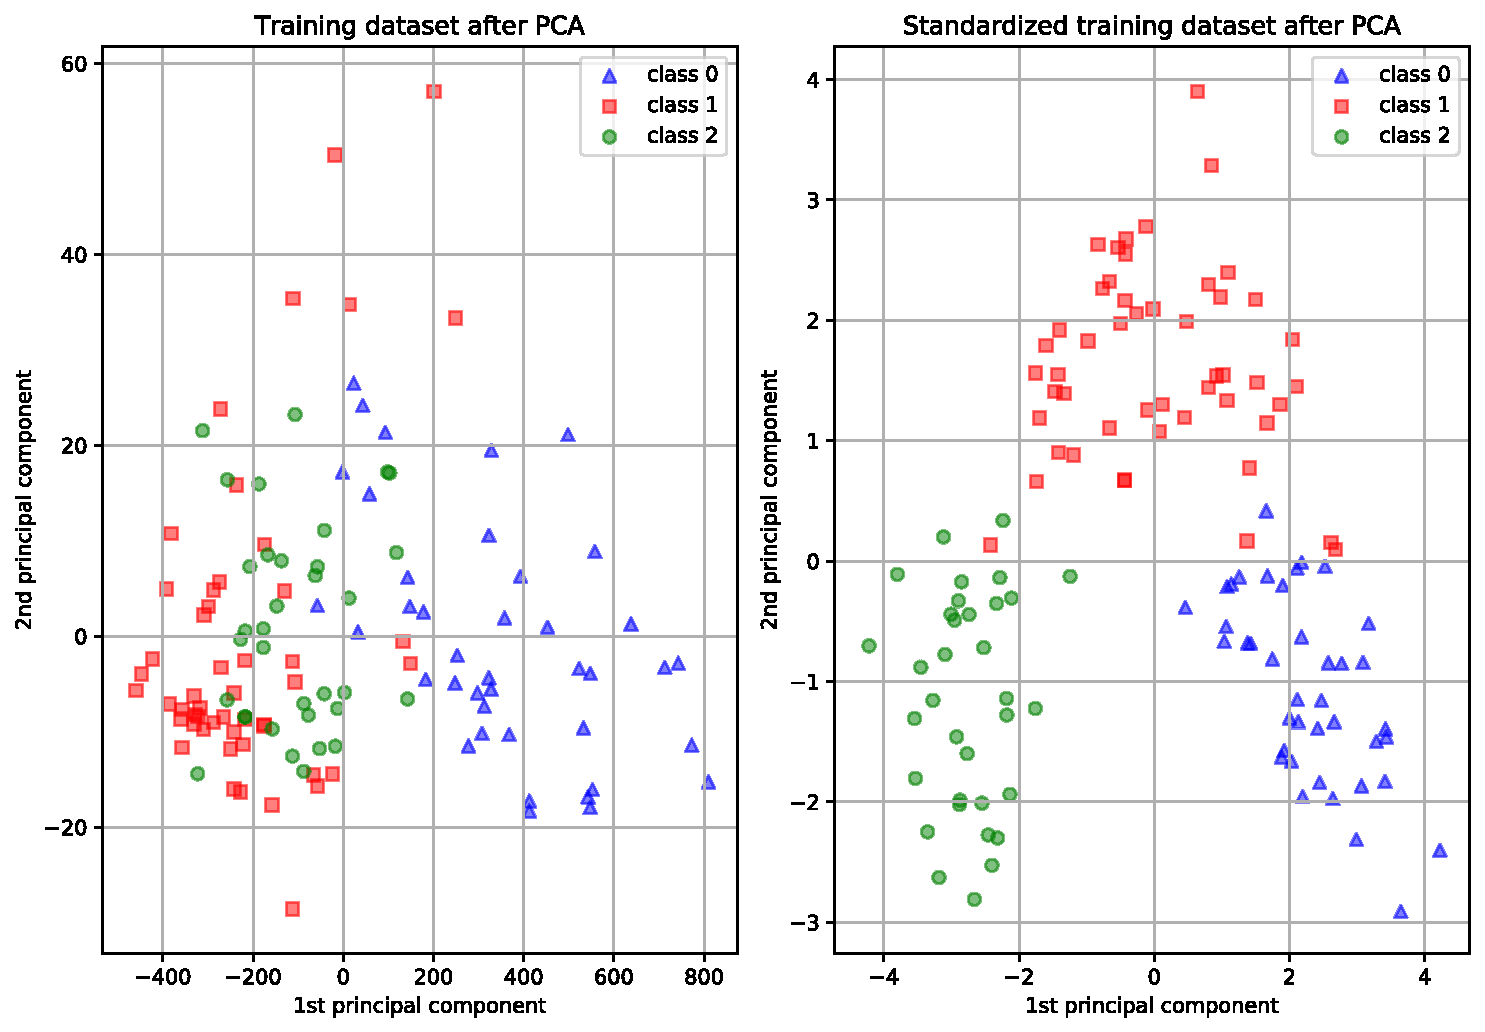
\includegraphics[width=0.8\linewidth]{contents/chapter_4/resources/example_pca_scaling.pdf}
    \caption{Exemple de l'impact de la distribution de données sur le \gls{pca} appliqué à une analyse chimique du vin en provenance de différentes région~\textsuperscript{\ref{footnote:exemple_pca_scaling}}. A gauche, le résultat issu du \gls{pca} sans normalisation préalable; A droite, la distribution après normalisation et \gls{pca}.}
    \label{fig:exemple_pca_scaling}
\end{figure}\par

\addtocounter{footnote}{1}
\footnotetext[\thefootnote]{Source : Scikit-learn - \href{https://scikit-learn.org/stable/auto_examples/preprocessing/plot_scaling_importance.html}{"Importance of Feature Scaling"}. \label{footnote:exemple_pca_scaling}}

Divers travaux ont ainsi été menés, afin de proposer des méthodes de normalisation à cette problématique. L'un de ces travaux propose trois méthodes de normalisation par la variance, par le maximum, et par le minimum et maximum dans le contexte de \gls{svm}~\cite{Juszczak2002}. Ces trois méthode semblent ainsi propice à réduire l'erreur de classification. Le travail mené par Celebi et al.~\cite{Celebi2007}, propose une normalisation des caractéristiques à l'aide de la "Cote Z" ou "Standard score", c'est à dire par soustraction de la moyenne au sein d'un même groupe de caractéristiques puis par division de l'écart type de ce même groupe.\par

Afin de couvrir au mieux la problématique de la normalisation, nous traiterons cette problématique sous trois méthodes majeures:
\begin{itemize}
    \item l'utilisation de la normalisation "Min-Max"~\cite{Juszczak2002},
    \item l'utilisation de la normalisation "Standard"~\cite{Celebi2007}, 
    \item et l'utilisation de la normalisation "Robust". 
\end{itemize}
Ces diverses méthode de normalisation seront évalué face à un processus n'employant aucune d'entre elles, nous servant ainsi de méthode de comparaison. De plus ces méthodes seront réalisées en amont du processus de pré traitement afin de couvrir également les méthodes de réduction de l'information pouvant être affectées. L'\Cref{eq:scaling_methods} couvre les diverses équations listé précédemment.\par

\begin{equation} 
    \label{eq:scaling_methods}
    \begin{split}
    &MinMax=\frac{X-min(X)}{max(X)-min(X)}  \\
    &Standard=\frac{X-\mu{}}{\sigma}	    \\
    &Robust=\frac{xi–Q1(x)}{Q3(x)–Q1(x)}    \\
    \end{split}
\end{equation}

\subsection{Balancement de caractéristiques}
L'une des problématiques associés de manière récurrente aux problématiques d'apprentissage sur des données réelles, en opposition avec des données provenant de modèle génératifs par exemple, est celle de la répartition homogène des annotations. Ces déséquilibres pouvant survenir au sein des annotations sont qualifié sous le terme anglais de "class imbalancement"~\cite{Prati2009, He2009}.\par

Cette problématique est récurrente à de nombreux domaines d'applications, mais touche essentiellement les domaines où la tâche visée correspond à la détection d'événements isolés au sein d'une population, comme par exemple: 
\begin{inlinerate}
    \item les comportements déviants (fraude bancaire~\cite{Phua2004}),
    \item le respect de critère de qualité (vérification de pièces industrielles~\cite{Wu2018}),
    \item ou encore dans notre domaine d'anormalités clinique (cancers ou d'autres pathologies cliniques~\cite{Celebi2007}),
    \item \ldots
\end{inlinerate}\par

Certains choix peuvent permettre de limiter l'impact d'un déséquilibre d'annotations. Ainsi, la sélection d'un métrique adéquate peux permettre de limiter la dépendance au données: la substitution de la précision par des mesures telles que l'\gls{auc}~\cite{Celebi2007} ou le f1-score sont des solutions pertinentes dans de telles situations. Néanmoins, la plupart des modèles de classification échouerons à classifier convenablement les données dans des situations de fort déséquilibres. Ces modèles préférerons prédire constamment la classe majoritaire, pour minimiser le coût de l'erreur~\cite{Huang2013}. Dans le cadre de modèles basés sur des arbres de décision, la stratégie générale propose de déterminer les critères majeurs de séparation par partitionnement successif des données. Ce partitionnement conduit inéluctablement à un affaiblissement des classes minoritaires~\cite{He2009}.\par 

Afin de corriger ces éléments, deux catégories d'approches ont été proposées pour solutionner ce déséquilibre~\cite{Huang2013}. Les approches par corrections de donnée procède par augmentation ou décimations de ces dernières afin de rééquilibré les annotations. Les approches algorithmiques consistent à pondérer la valeur des annotations afin de prendre en considération le déséquilibre d'information~\cite{Ting2002,He2009,Thai2010}.\par

En premier lieu, des approches par correction des données simples, proposes diverses solutions pour palier à ces déséquilibres de classes~\cite{Prati2009, He2009}. Une première catégories de ces méthodes consiste à \textbf{sous-échantillonner} les données jusqu'à obtenir une égalité entre les classes. Son principe le plus simple est celui du "Sous-échantillonage aléatoire" consistant à décimer de manière aléatoire les données des classes majoritaire afin d'égaler les échantillons de la classe minoritaire. A l'inverse, une autre catégorie consiste à \textbf{sur-échantillonner} les données possédées afin d'obtenir à nouveau une égalité entre classes. Le principe le plus simples est celui du "Sur-échantillonage aléatoire" consistant à dupliquer aléatoirement les échantillons des classes minoritaires afin d'égaler le nombre d'élément de la classe majoritaire. Le schéma en \Cref{fig:scheme_data_balancing} reprendre l'idée de ces deux principes.\par

\begin{figure}[H]
    \centering
    \includegraphics[width=\linewidth]{contents/chapter_4/resources/scheme_data_balancing.pdf}
    \caption{Schéma des deux stratégies principales de balancement de données. A gauche, la stratégie de sous-échantillonage, dans laquelle des éléments sont aléatoirement choisis jusqu'à réduire l'ensemble des classes au nombre d'éléments de la classe minoritaire; A droite, la stratégie de sur-échantillonage, dans laquelle les éléments des classes minoritaires sont dupliqués aléatoirement. }
    \label{fig:scheme_data_balancing}
\end{figure}\par

En second lieu, des approches par correction des données plus avancées ont été proposées. De manière non exhaustive nous proposerons l'une d'entre elle pour chaque catégories:
\begin{itemize}
    \item par \textbf{sous-échantillonnage}: \cite{Tomek1976}
    \item par \textbf{sur-échantillonnage}:\cite{Chawla2002} 
    \item par \textbf{combinaison}: SMOTE + Tomek
    \item \ldots
\end{itemize}\par

Les approches algorithmique par pondération, consiste à considérer le non balancement de l'information en pondérant l'importance de chaque échantillon lors de l'apprentissage du modèle.  

Dans l'optique de récapituler cette partie, les méthodes utilisées dans le but de corriger le déséquilibre des données sont référencée dans la \Cref{tab:summary_balancement_methods}. Afin de traiter au mieux cette tâche, la balancement de données par ses différentes stratégies évoquée sera réalisé avec l'aide de la librairie logicielle "Imbalanced-learn"~\cite{Lemaitre2017}. La correction par algorithme, plus précisément pondération, sera réalisé avec l'aide de la bibliothèque "Scikit-learn"~\cite{pedregosa2011}.\par

\begin{table}[H]
    \centering
    \begin{tabular*}{0.6\linewidth}{l@{\extracolsep{\fill}}l}
    \toprule
    \textbf{Catégorie}                  & \textbf{Méthode}                  \\ \hline
    \multirow{2}{*}{Sous-échantillonage}& Sous-échantillonage aléatoire     \\ \cline{2-2}
                                        & Tomek Link                        \\ \hline
    \multirow{2}{*}{Sur-échantillonage} & Sur-échantillonage aléatoire      \\ \cline{2-2}
                                        & SMOTE                             \\ \hline
    Combinaison                         & SMOTE + Tomek                     \\ \hline 
    Algorithme                          & Pondération                       \\
    \bottomrule
    \end{tabular*}
    \caption{Liste des diverses méthodes de balancement mises en oeuvre pour corriger les déséquilibre de données.}
    \label{tab:summary_balancement_methods}
\end{table}\par

\subsection{Réduction de dimensions}
Dans le domaine de l'apprentissage automatique, la réduction de dimension est une technique qui permet de réduire l'information extraites afin de rendre un problème moins complexe. Également, elle est un moyen de se prévenir du "Fléau de la dimension", phénomène qui met en perspective d'une part la croissance exponentielle de l'ajout de nouvelles dimensions à la dilution des divers échantillons dans cet espace. Ce dilemme a pour principales conséquences d'augmenter la complexité d'un problème, la durée nécessaire à sa résolution mais également d'engendrer des risques de sur-apprentissage.\par

A cette fin, deux catégories de méthodes cohabitent: d'une part les méthode de sélection de caractéristiques, qui réduise l'espace en décimant certaine dimension jugées non pertinente à la résolution du problème; d'autre part les méthode par projection ou transformation de l'espace existant qui réduisent et modifie les valeurs existantes. Notre investigation ne portera que sur cette seconde catégorie de méthodes.\par

pca\par
lda\par~\cite{Nanni2017}


\section{Méthodes de prédiction}

\section{Processus et metriques}
\section{Résultats}


Néanmoins, il est également a été également jugées important de l'intersection d'évènements tels que la présence de tissus caractéristiques aux abords de follicules pileux.\par